\chapter{Equilibrium p--n Junction and Depletion Electrostatics}
\label{ch:equilibrium-pn-junction}

The previous chapters established equilibrium carrier statistics, drift,
diffusion, recombination, and high-field transport in homogeneous material.  A
p--n junction joins regions with different equilibrium chemical potentials.
Carrier diffusion then creates a space-charge layer, an electric field, and a
built-in electrostatic potential.  This chapter follows the physical sequence
of Sze and Lee: thermal equilibrium, space charge, Poisson's equation, abrupt
and graded depletion regions, and applied bias \cite[Chap.~3, Secs.~3.1--3.2]{szeLee2012}.

\section{Notation and voltage convention}

\begin{center}
\small
\begin{tabularx}{\textwidth}{@{}lX@{}}
\toprule
Symbol & Meaning and SI unit unless stated otherwise \\
\midrule
$N_A,N_D,n_i$ & Ionized acceptor density, ionized donor density, and intrinsic carrier density, each in $\mathrm{m^{-3}}$. \\
$n,p$ & Electron and hole densities in $\mathrm{m^{-3}}$. \\
$q,\kb,T,V_T$ & Positive elementary charge in coulombs, Boltzmann constant, absolute temperature in kelvin, and thermal voltage $V_T=\kb T/q$ in volts. \\
$\psi,E,\varepsilon_s$ & Electrostatic potential in volts, electric field $E=-\dd\psi/\dd x$ in $\mathrm{V\,m^{-1}}$, and semiconductor permittivity in $\mathrm{F\,m^{-1}}$. \\
$V_{\mathrm{bi}},V$ & Built-in potential and applied junction voltage in volts; $V>0$ denotes forward bias. \\
$x_p,x_n,W$ & Depletion widths on the p-side, on the n-side, and in total, measured in meters. \\
$\rho,E_m$ & Volume charge density in $\mathrm{C\,m^{-3}}$ and maximum field magnitude in $\mathrm{V\,m^{-1}}$. \\
\bottomrule
\end{tabularx}
\end{center}

\begin{definition}{Metallurgical and electrical junctions}{pn-junction}
The \emph{metallurgical junction} is the surface at which the net dopant type
changes sign.  The \emph{electrical junction} is the space-charge region and
its surrounding transition layers.  Their locations need not coincide in a
nonabrupt or processed device.
\end{definition}

\section{Contact, diffusion, and thermal equilibrium}

\subsection{Before contact}

Consider two homogeneous pieces of the same nondegenerate semiconductor with
complete dopant ionization before they are allowed to exchange carriers.

\paragraph{n-type region.}
In the neutral n-type piece, the electron concentration is approximately the
donor density, while the hole concentration follows from mass action:
\begin{equation}
 n_n\simeq N_D,
 \qquad
 p_n=\frac{n_i^2}{n_n}\simeq\frac{n_i^2}{N_D},
 \qquad
 E_C-E_{F,n}=\kb T\ln\!\left(\frac{N_C}{N_D}\right).
 \label{eq:pn-isolated-n-region}
\end{equation}
The large electron population places $E_{F,n}$ near the conduction-band edge.

\paragraph{p-type region.}
In the neutral p-type piece, the hole concentration is approximately the
acceptor density, while the electron concentration follows from mass action:
\begin{equation}
 p_p\simeq N_A,
 \qquad
 n_p=\frac{n_i^2}{p_p}\simeq\frac{n_i^2}{N_A},
 \qquad
 E_{F,p}-E_V=\kb T\ln\!\left(\frac{N_V}{N_A}\right).
 \label{eq:pn-isolated-p-region}
\end{equation}
The large hole population places $E_{F,p}$ near the valence-band edge.

With both pieces expressed in one common band-energy reference,
\begin{equation}
 E_{F,n}-E_{F,p}
 =\kb T\ln\!\left(\frac{N_A N_D}{n_i^2}\right).
 \label{eq:pn-isolated-fermi-separation}
\end{equation}
Each isolated piece is internally in thermal equilibrium, but the two pieces
are not in \emph{mutual} diffusive equilibrium: their chemical potentials
are different and carrier exchange has not yet been permitted.

Band alignment before contact requires careful language.  Independent isolated
bodies have arbitrary electrostatic-potential zeros, so an absolute statement
that their $E_C$ and $E_V$ values are aligned or misaligned is meaningless
until a common energy reference is chosen.  For a homojunction made from the
same semiconductor and drawn on a common vacuum-energy reference, the band
edges align while the Fermi levels differ, as in
\cref{fig:junction-atlas-formation}.  A different choice of potential zero can
rigidly shift all three energies of either isolated piece without changing any
physics.  Within each uniform neutral piece the bands are flat, and therefore
no internal electric field exists before contact.

\subsection{After contact and equilibrium}

After contact, electrons diffuse from n to p and holes diffuse from p to n.
Recombination removes part of this mobile charge near the interface.  The
uncovered ionized acceptors are negative; the uncovered ionized donors are
positive.  Their field points from n to p and opposes further majority-carrier
diffusion.

Thermal equilibrium is reached when drift and diffusion cancel separately for
electrons and holes.  Setting the electron current to zero gives
\begin{equation}
  J_n=q\mu_n nE+qD_n\frac{\dd n}{\dd x}=0.
  \label{eq:pn-equilibrium-electron-current}
\end{equation}
Using $D_n/\mu_n=V_T$ and the nondegenerate relation between $n$ and the band
edge shows that the Fermi energy is independent of position.  The same result
follows from $J_p=0$.  A flat Fermi level is therefore the diagnostic of
thermal equilibrium, whereas the band edges bend with $-q\psi(x)$.

For completely ionized, nondegenerate neutral regions,
\begin{equation}
  \boxed{
  V_{\mathrm{bi}}=V_T\ln\!\left(\frac{N_A N_D}{n_i^2}\right).
  }
  \label{eq:pn-built-in-potential}
\end{equation}
More generally, if an equilibrium calculation supplies isolated n-type and
p-type chemical potentials in one common band-energy reference, then
\begin{equation}
 qV_{\mathrm{bi}}
 =\mu_n^{\mathrm{bulk}}-\mu_p^{\mathrm{bulk}}.
 \label{eq:pn-built-in-from-bulk-chemical-potentials}
\end{equation}
This form remains the correct starting point when incomplete ionization or
compensation makes $n\ne N_D$ or $p\ne N_A$.  A common rigid shift of both
chemical potentials cancels from their difference.  Chapter~\ref{ch:equilibrium-to-device-prediction}
develops the corresponding data-transfer and validation procedure.

The contact potential is an internal equilibrium quantity.  A voltmeter does
not read $V_{\mathrm{bi}}$ directly because contact potentials at the external
terminals complete the electrochemical-potential balance.

\begin{figure}[htbp]
 \centering
 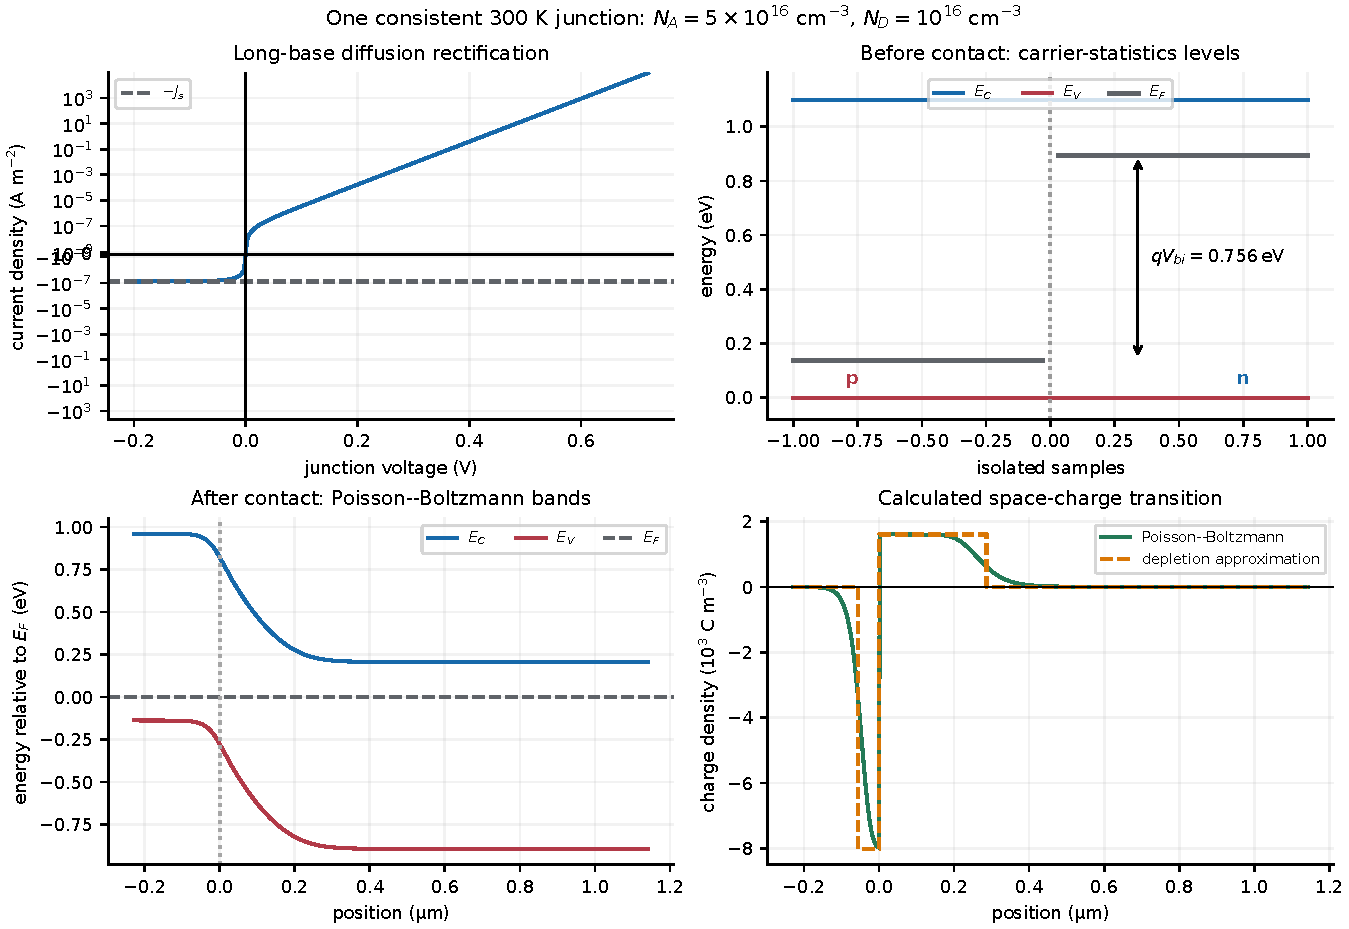
\includegraphics[width=\textwidth]{figures/junction-atlas-formation.pdf}
 \caption{Parameter-consistent calculation for a Si-like abrupt junction with
 $N_A=5\times10^{16}\,\mathrm{cm^{-3}}$, $N_D=10^{16}\,\mathrm{cm^{-3}}$,
 $n_i=10^{10}\,\mathrm{cm^{-3}}$, and $T=300\,\mathrm K$.  The rectifying
 current uses the long-base minority-diffusion model with
 $\mu_n=1350\,\mathrm{cm^2\,V^{-1}\,s^{-1}}$,
 $\mu_p=480\,\mathrm{cm^2\,V^{-1}\,s^{-1}}$, and
 $\tau_n=\tau_p=\SI{1}{\micro\second}$; the isolated Fermi levels
 follow effective-density-of-states statistics; and the contacted band edges
 and smooth space charge come from the nonlinear Poisson--Boltzmann solution.
 The dashed charge profile is the depletion approximation for the same device.
 These panels cover the physical content introduced in Figs.~1--3 of Sze--Lee
 Chapter~3 \cite[Sec.~3.1]{szeLee2012}.\figurenotebookmark}
 \label{fig:junction-atlas-formation}
\end{figure}
\figurenotebooktext{figures/16_equilibrium-pn-junction/fig_16_01.ipynb}

\section{Poisson equation and the depletion approximation}

The exact one-dimensional charge density is
\begin{equation}
  \rho(x)=q\bigl[p(x)-n(x)+N_D^+(x)-N_A^-(x)\bigr],
  \label{eq:pn-exact-charge-density}
\end{equation}
where the superscripts emphasize that depletion charge is set by ionized
rather than nominal dopant density.  Complete ionization replaces
$N_D^+,N_A^-$ by $N_D,N_A$.  A frozen-ionization approximation instead imports
the homogeneous bulk values.  A local-equilibrium model recalculates dopant
occupation as the bands bend and must retain $N_D^+(x)$ and $N_A^-(x)$ inside
the nonlinear Poisson solve.

Electrostatics requires
\begin{equation}
  \frac{\dd E}{\dd x}=\frac{\rho}{\varepsilon_s},
  \qquad
  \frac{\dd^2\psi}{\dd x^2}=-\frac{\rho}{\varepsilon_s}.
  \label{eq:pn-poisson}
\end{equation}

\begin{definition}{Depletion approximation}{depletion-approximation}
The depletion approximation neglects mobile $n$ and $p$ inside the space-charge
region, retains the fixed ionized dopants there, and sets net charge to zero in
the quasi-neutral regions.  It replaces smooth transition layers by sharp
edges at $x=-x_p$ and $x=x_n$.
\end{definition}

For an abrupt junction at $x=0$,
\begin{equation}
 \rho(x)=
 \begin{cases}
  -qN_A,&-x_p<x<0,\\
  +qN_D,&0<x<x_n,\\
  0,&\text{otherwise}.
 \end{cases}
 \label{eq:pn-abrupt-charge}
\end{equation}
Zero field in both neutral bulks requires total depletion charge to vanish:
\begin{equation}
  \boxed{N_Ax_p=N_Dx_n.}
  \label{eq:pn-charge-neutrality}
\end{equation}
Thus the lower-doped side supports the greater depletion width.

Integrating Poisson's equation gives a triangular field.  Its maximum magnitude
at the metallurgical junction is
\begin{equation}
  E_m=\frac{qN_Ax_p}{\varepsilon_s}
     =\frac{qN_Dx_n}{\varepsilon_s}.
  \label{eq:pn-maximum-field}
\end{equation}
The area under $-E(x)$ is the depletion potential.  Under applied junction
voltage $V$, this drop is $V_{\mathrm{bi}}-V$, so
\begin{align}
  W&=x_p+x_n
  =\sqrt{\frac{2\varepsilon_s}{q}(V_{\mathrm{bi}}-V)
  \left(\frac{1}{N_A}+\frac{1}{N_D}\right)},
  \label{eq:pn-abrupt-width}\\
  x_p&=\frac{N_D}{N_A+N_D}W,
  \qquad
  x_n=\frac{N_A}{N_A+N_D}W.
  \label{eq:pn-width-partition}
\end{align}
Forward bias lowers the barrier and narrows the layer.  Reverse bias, $V<0$,
raises the barrier and widens it.

\section{One-sided and graded junctions}

If $N_A\gg N_D$, then $x_p\ll x_n$ and $W\simeq x_n$.  This one-sided
$p^+$--n limit reduces \cref{eq:pn-abrupt-width} to
\begin{equation}
  W\simeq\sqrt{\frac{2\varepsilon_s(V_{\mathrm{bi}}-V)}{qN_D}}.
  \label{eq:pn-one-sided-width}
\end{equation}
The lightly doped region controls width, capacitance, and peak field.

A linearly graded junction instead has net doping
$N_D-N_A=ax$, where $a$ is the impurity gradient in $\mathrm{m^{-4}}$.  A
symmetric depleted interval of width $W$ contains $\rho=qax$, giving
\begin{equation}
  V_{\mathrm{bi}}-V=\frac{qaW^3}{12\varepsilon_s},
  \qquad
  W=\left[\frac{12\varepsilon_s(V_{\mathrm{bi}}-V)}{qa}\right]^{1/3}.
  \label{eq:pn-graded-width}
\end{equation}
The $1/3$ exponent distinguishes graded from abrupt junctions.

\begin{figure}[htbp]
 \centering
 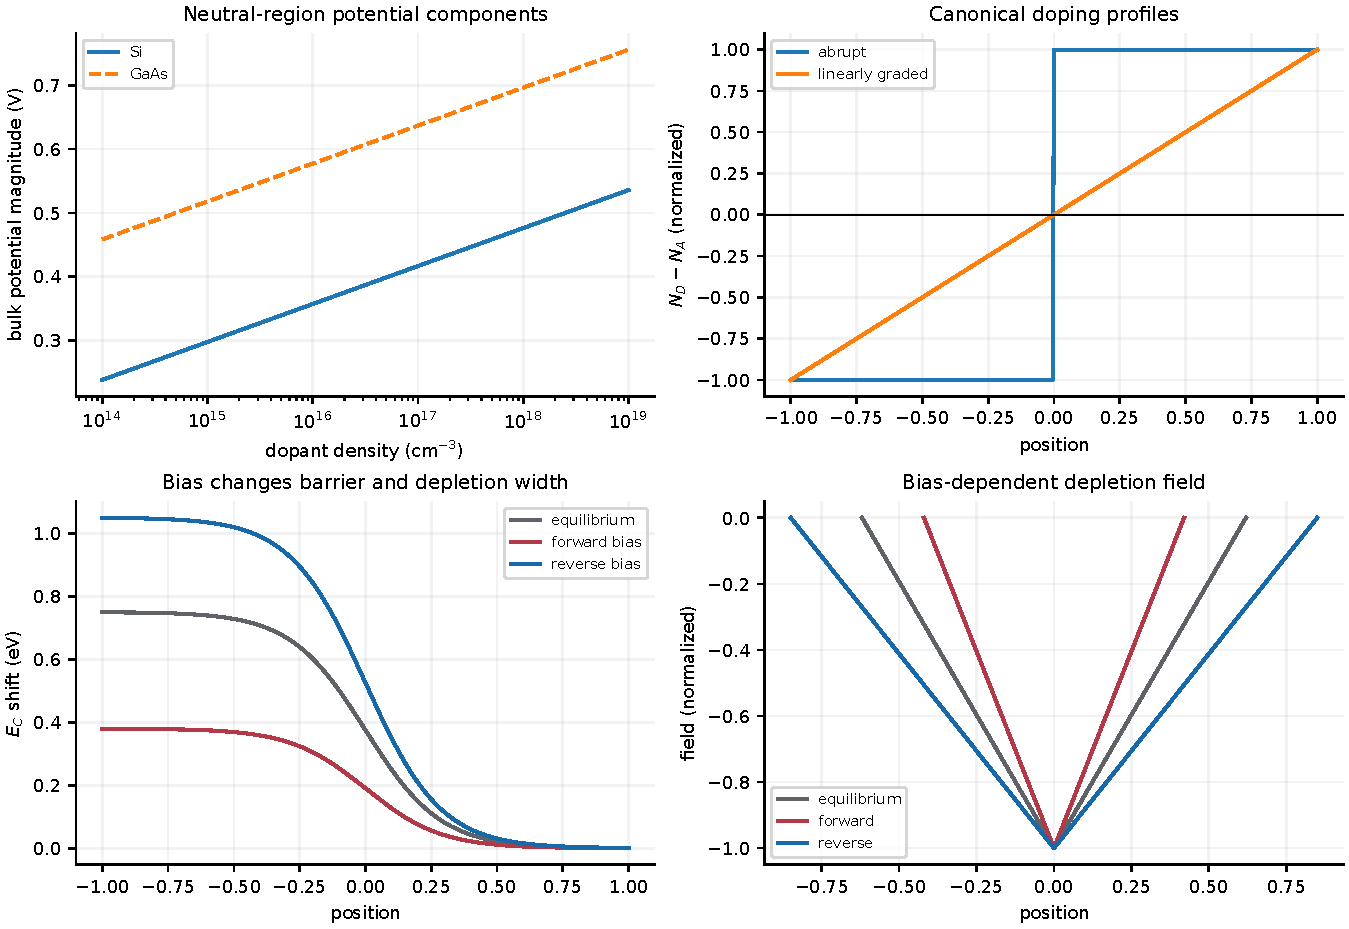
\includegraphics[width=\textwidth]{figures/junction-atlas-doping-bias.pdf}
 \caption{Original plots of neutral-region potential components, abrupt and
 graded doping profiles, and barrier and field changes under equilibrium,
 forward bias, and reverse bias.  They reproduce the physical comparisons of
 Figs.~4, 5, and 8 in Sze--Lee Chapter~3 from the chapter equations rather than
 from scanned artwork \cite[Secs.~3.1--3.2]{szeLee2012}.\figurenotebookmark}
 \label{fig:junction-atlas-doping-bias}
\end{figure}
\figurenotebooktext{figures/16_equilibrium-pn-junction/fig_16_01.ipynb}

\begin{figure}[htbp]
 \centering
 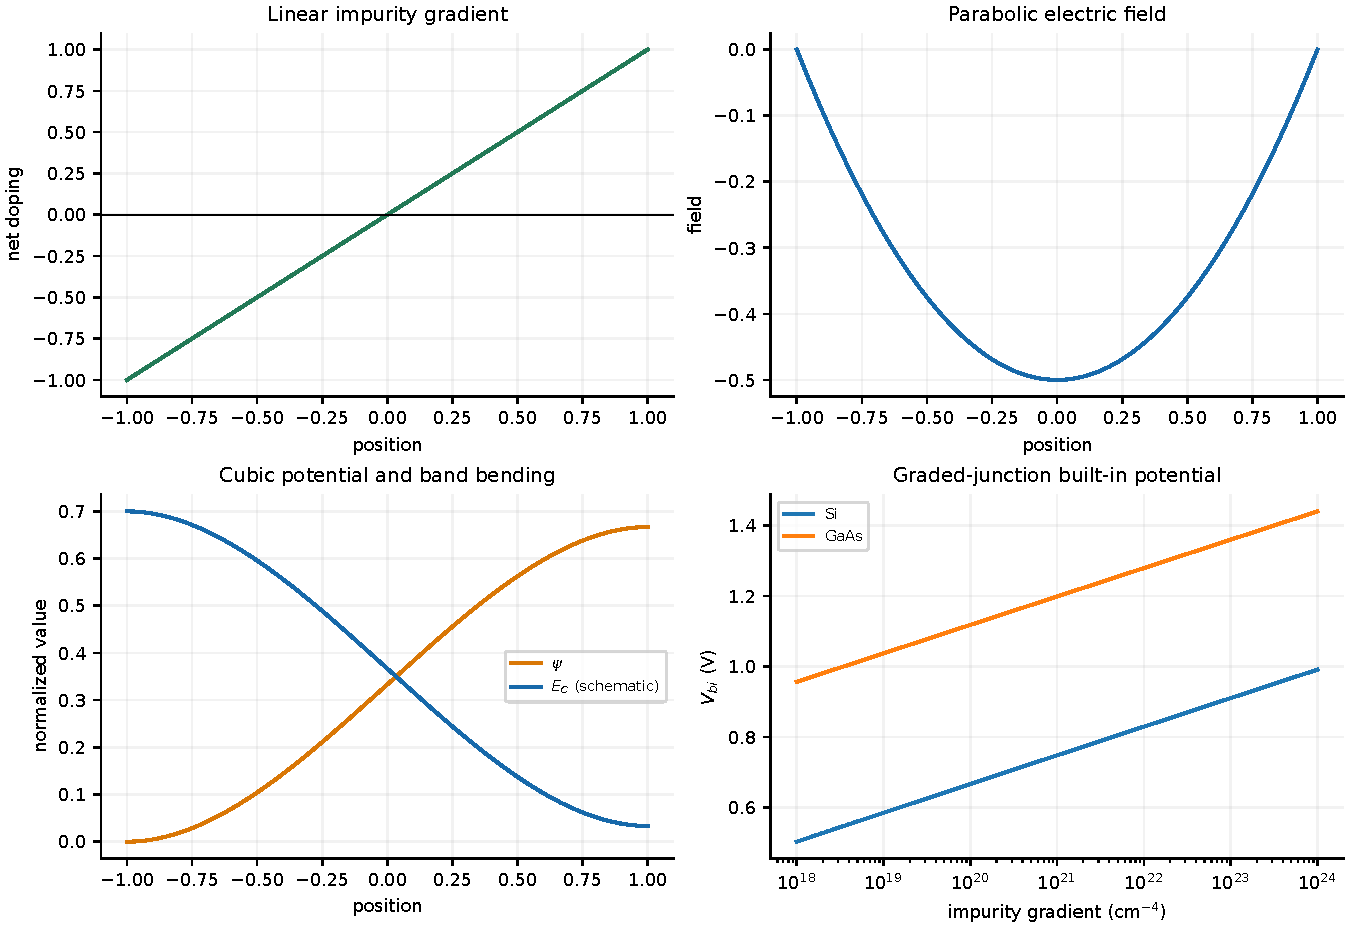
\includegraphics[width=\textwidth]{figures/junction-atlas-graded.pdf}
 \caption{Linearly graded impurity density, parabolic field, cubic potential,
 band bending, and the calculated built-in-potential trend for Si and GaAs.
 The panels cover the subjects of Figs.~9--10 in Sze--Lee Chapter~3
 \cite[Sec.~3.2.2]{szeLee2012}.\figurenotebookmark}
 \label{fig:junction-atlas-graded}
\end{figure}
\figurenotebooktext{figures/16_equilibrium-pn-junction/fig_16_01.ipynb}

\section{Finite-difference Poisson--Boltzmann validation}

The depletion approximation should be compared with an equilibrium solution
that retains mobile carriers.  For an abrupt fully ionized junction,
\begin{equation}
 n=n_i e^{\psi/V_T},\qquad p=n_i e^{-\psi/V_T}.
 \label{eq:pn-boltzmann-carriers}
\end{equation}
On a uniform grid $x_i$, the nonlinear interior equation is
\begin{equation}
 \frac{\psi_{i-1}-2\psi_i+\psi_{i+1}}{\Delta x^2}
 =-\frac{q}{\varepsilon_s}
 \left[n_i e^{-\psi_i/V_T}-n_i e^{\psi_i/V_T}+N_D-N_A\right]_i.
 \label{eq:pn-poisson-fd}
\end{equation}
Neutral-bulk Dirichlet conditions follow from
$n-p=N_D-N_A$:
\begin{equation}
 \psi_{\mathrm{bulk}}
 =V_T\operatorname{asinh}\!\left(\frac{N_D-N_A}{2n_i}\right).
 \label{eq:pn-neutral-boundary-potential}
\end{equation}
A damped nonlinear root solve produces the smooth charge transition omitted by
the depletion model.  The potential drop and integrated charge remain the
strong validation quantities.

\begin{figure}[htbp]
 \centering
 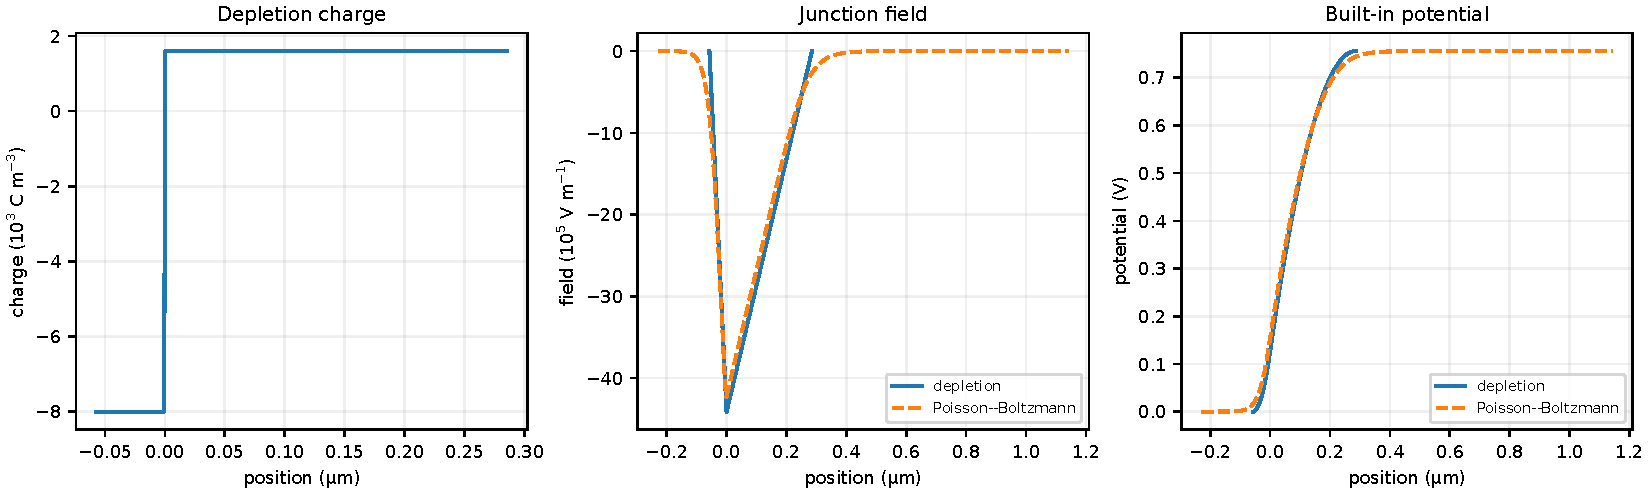
\includegraphics[width=\textwidth]{figures/junction-equilibrium-depletion.pdf}
 \caption{Abrupt-junction depletion charge, electric field, and potential,
 compared with a nonlinear finite-difference Poisson--Boltzmann solution.  The
 depletion model captures the integrated electrostatics while replacing smooth
 mobile-carrier transition layers by sharp boundaries; these are the
 electrostatic subjects of Figs.~6--7 in Sze--Lee Chapter~3
 \cite[Sec.~3.2.1]{szeLee2012}.\figurenotebookmark}
 \label{fig:junction-equilibrium-depletion}
\end{figure}
\figurenotebooktext{figures/16_equilibrium-pn-junction/fig_16_01.ipynb}

\begin{modelcheck}
For $N_A=5\times10^{22}\,\mathrm{m^{-3}}$,
$N_D=10^{22}\,\mathrm{m^{-3}}$, $n_i=10^{16}\,\mathrm{m^{-3}}$, and
$T=300\,\mathrm K$, \cref{eq:pn-built-in-potential} gives
$V_{\mathrm{bi}}=0.756\,\mathrm V$.  The finite-difference boundary-potential
difference agrees with this value, its normalized nonlinear residual is below
$10^{-10}$, and the depletion charges satisfy $N_Ax_p=N_Dx_n$.
\end{modelcheck}

\begin{boundarybox}
The present equations assume nondegenerate Boltzmann statistics, complete
ionization, uniform permittivity, one-dimensional geometry, and no interface
charge.  Heavy doping requires Fermi--Dirac statistics and band-gap narrowing.
Nanometer junctions can require quantum confinement and tunneling.  Junction
curvature requires two- or three-dimensional Poisson electrostatics.
\end{boundarybox}

\section{Chapter summary}

Carrier diffusion across a newly formed p--n junction exposes fixed dopant
charge.  The resulting field balances diffusion and makes the equilibrium
Fermi level spatially constant.  Charge neutrality partitions the depletion
width between the two sides, and Poisson integration determines field,
potential, and bias response.  A nonlinear Poisson--Boltzmann calculation
shows precisely which smooth transition layers the depletion approximation
removes.
